\documentclass{standalone}
\usepackage{tikz}
\usetikzlibrary{patterns, positioning}
\usepackage[sfdefault]{ClearSans} %% option 'sfdefault' activates Clear Sans as the default text font
\usepackage[T1]{fontenc}

\begin{document}
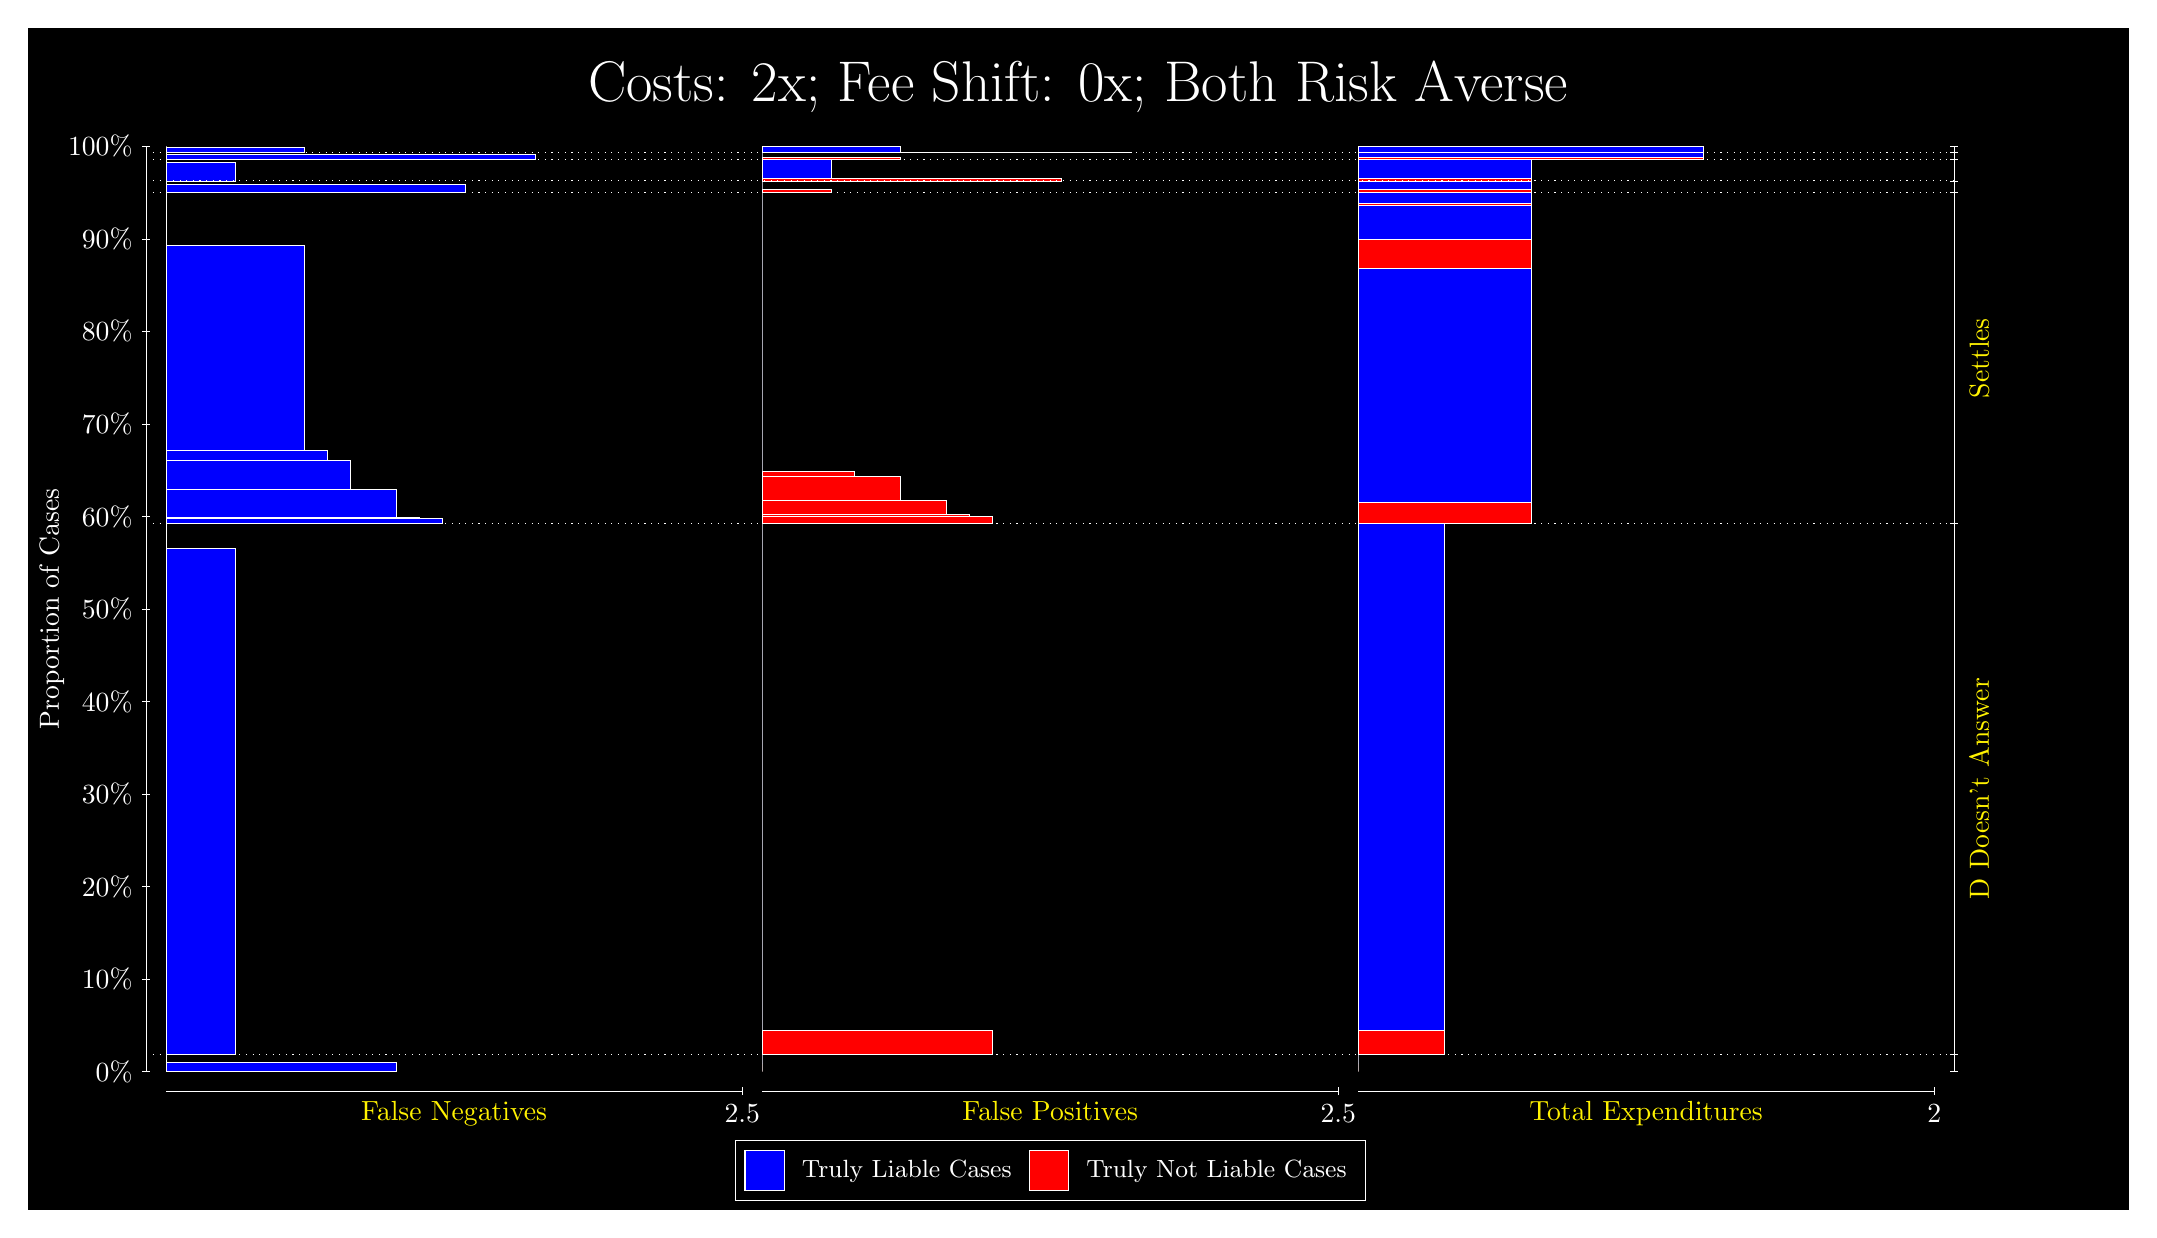
\begin{tikzpicture}
\draw[fill=black] (0,0) rectangle (26.667,15);
\draw[text=white] (0,13.5) rectangle (26.667,15) node[midway] {\huge Costs: 2x; Fee Shift: 0x; Both Risk Averse};
\draw[white, very thin] (1.5,1.75) -- (1.5,13.5);
\node[rotate=90, text=white, anchor=center] at (0.3, 7.625) {Proportion of Cases};
\draw[white, very thin] (1.45,1.75) -- (1.55,1.75);
\node[text=white, anchor=east] at (1.45, 1.75) {0\%};
\draw[white, very thin] (1.45,2.925) -- (1.55,2.925);
\node[text=white, anchor=east] at (1.45, 2.925) {10\%};
\draw[white, very thin] (1.45,4.1) -- (1.55,4.1);
\node[text=white, anchor=east] at (1.45, 4.1) {20\%};
\draw[white, very thin] (1.45,5.275) -- (1.55,5.275);
\node[text=white, anchor=east] at (1.45, 5.275) {30\%};
\draw[white, very thin] (1.45,6.45) -- (1.55,6.45);
\node[text=white, anchor=east] at (1.45, 6.45) {40\%};
\draw[white, very thin] (1.45,7.625) -- (1.55,7.625);
\node[text=white, anchor=east] at (1.45, 7.625) {50\%};
\draw[white, very thin] (1.45,8.8) -- (1.55,8.8);
\node[text=white, anchor=east] at (1.45, 8.8) {60\%};
\draw[white, very thin] (1.45,9.975) -- (1.55,9.975);
\node[text=white, anchor=east] at (1.45, 9.975) {70\%};
\draw[white, very thin] (1.45,11.15) -- (1.55,11.15);
\node[text=white, anchor=east] at (1.45, 11.15) {80\%};
\draw[white, very thin] (1.45,12.325) -- (1.55,12.325);
\node[text=white, anchor=east] at (1.45, 12.325) {90\%};
\draw[white, very thin] (1.45,13.5) -- (1.55,13.5);
\node[text=white, anchor=east] at (1.45, 13.5) {100\%};

\draw[white, very thin] (24.457,1.75) -- (24.457,13.5);
\draw[white, very thin] (24.407,1.75) -- (24.507,1.75);
\node[anchor=west] at (24.407, 1.75) {};
\draw[white, very thin] (24.407,1.9687) -- (24.507,1.9687);
\node[anchor=west] at (24.407, 1.9687) {};
\draw[white, very thin] (24.407,8.709) -- (24.507,8.709);
\node[anchor=west] at (24.407, 8.709) {};
\draw[white, very thin] (24.407,12.912) -- (24.507,12.912);
\node[anchor=west] at (24.407, 12.912) {};
\draw[white, very thin] (24.407,13.061) -- (24.507,13.061);
\node[anchor=west] at (24.407, 13.061) {};
\draw[white, very thin] (24.407,13.334) -- (24.507,13.334);
\node[anchor=west] at (24.407, 13.334) {};
\draw[white, very thin] (24.407,13.42) -- (24.507,13.42);
\node[anchor=west] at (24.407, 13.42) {};
\draw[white, very thin] (24.407,13.5) -- (24.507,13.5);
\node[anchor=west] at (24.407, 13.5) {};

\draw[white, very thin, fill=blue] (1.75,1.75) rectangle (4.6775,1.8718);
\draw[white, very thin, fill=red] (1.75,1.8718) rectangle (1.75,1.9687);
\draw[white, very thin, fill=blue] (1.75,1.9687) rectangle (2.6283,8.4005);
\draw[white, very thin, fill=red] (1.75,8.4005) rectangle (1.75,8.709);
\draw[white, very thin, fill=blue] (1.75,8.709) rectangle (5.2631,8.7792);
\draw[white, very thin, fill=blue] (1.75,8.7792) rectangle (4.9703,8.7829);
\draw[white, very thin, fill=blue] (1.75,8.7829) rectangle (4.6775,9.1431);
\draw[white, very thin, fill=blue] (1.75,9.1431) rectangle (4.092,9.5121);
\draw[white, very thin, fill=blue] (1.75,9.5121) rectangle (3.7993,9.6452);
\draw[white, very thin, fill=blue] (1.75,9.6452) rectangle (3.5065,12.249);
\draw[white, very thin, fill=red] (1.75,12.249) rectangle (1.75,12.912);
\draw[white, very thin, fill=blue] (1.75,12.912) rectangle (5.5558,13.015);
\draw[white, very thin, fill=red] (1.75,13.015) rectangle (1.75,13.061);
\draw[white, very thin, fill=blue] (1.75,13.061) rectangle (2.6283,13.303);
\draw[white, very thin, fill=red] (1.75,13.303) rectangle (1.75,13.334);
\draw[white, very thin, fill=blue] (1.75,13.334) rectangle (6.4341,13.396);
\draw[white, very thin, fill=red] (1.75,13.396) rectangle (1.75,13.42);
\draw[white, very thin, fill=blue] (1.75,13.42) rectangle (3.5065,13.493);
\draw[white, very thin, fill=red] (1.75,13.493) rectangle (1.75,13.5);
\draw[white, very thin, fill=red] (9.3189,1.75) rectangle (9.3189,1.8468);
\draw[white, very thin, fill=blue] (9.3189,1.8468) rectangle (9.3189,1.9687);
\draw[white, very thin, fill=red] (9.3189,1.9687) rectangle (12.246,2.2772);
\draw[white, very thin, fill=blue] (9.3189,2.2772) rectangle (9.3189,8.709);
\draw[white, very thin, fill=red] (9.3189,8.709) rectangle (12.246,8.798);
\draw[white, very thin, fill=red] (9.3189,8.798) rectangle (11.954,8.8215);
\draw[white, very thin, fill=red] (9.3189,8.8215) rectangle (11.661,9.0074);
\draw[white, very thin, fill=red] (9.3189,9.0074) rectangle (11.075,9.3065);
\draw[white, very thin, fill=red] (9.3189,9.3065) rectangle (10.783,9.3089);
\draw[white, very thin, fill=red] (9.3189,9.3089) rectangle (10.49,9.3721);
\draw[white, very thin, fill=blue] (9.3189,9.3721) rectangle (9.3189,12.912);
\draw[white, very thin, fill=red] (9.3189,12.912) rectangle (10.197,12.957);
\draw[white, very thin, fill=blue] (9.3189,12.957) rectangle (9.3189,13.061);
\draw[white, very thin, fill=red] (9.3189,13.061) rectangle (13.125,13.091);
\draw[white, very thin, fill=blue] (9.3189,13.091) rectangle (10.197,13.334);
\draw[white, very thin, fill=red] (9.3189,13.334) rectangle (11.075,13.358);
\draw[white, very thin, fill=blue] (9.3189,13.358) rectangle (9.3189,13.42);
\draw[white, very thin, fill=red] (9.3189,13.42) rectangle (14.003,13.427);
\draw[white, very thin, fill=blue] (9.3189,13.427) rectangle (11.075,13.5);
\draw[white, very thin, fill=red] (16.888,1.75) rectangle (16.888,1.8468);
\draw[white, very thin, fill=blue] (16.888,1.8468) rectangle (16.888,1.9687);
\draw[white, very thin, fill=red] (16.888,1.9687) rectangle (17.986,2.2772);
\draw[white, very thin, fill=blue] (16.888,2.2772) rectangle (17.986,8.709);
\draw[white, very thin, fill=red] (16.888,8.709) rectangle (19.083,8.9838);
\draw[white, very thin, fill=blue] (16.888,8.9838) rectangle (19.083,11.956);
\draw[white, very thin, fill=red] (16.888,11.956) rectangle (19.083,12.321);
\draw[white, very thin, fill=blue] (16.888,12.321) rectangle (19.083,12.755);
\draw[white, very thin, fill=red] (16.888,12.755) rectangle (19.083,12.779);
\draw[white, very thin, fill=blue] (16.888,12.779) rectangle (19.083,12.912);
\draw[white, very thin, fill=red] (16.888,12.912) rectangle (19.083,12.957);
\draw[white, very thin, fill=blue] (16.888,12.957) rectangle (19.083,13.061);
\draw[white, very thin, fill=red] (16.888,13.061) rectangle (19.083,13.091);
\draw[white, very thin, fill=blue] (16.888,13.091) rectangle (19.083,13.334);
\draw[white, very thin, fill=red] (16.888,13.334) rectangle (21.279,13.358);
\draw[white, very thin, fill=blue] (16.888,13.358) rectangle (21.279,13.42);
\draw[white, very thin, fill=red] (16.888,13.42) rectangle (21.279,13.427);
\draw[white, very thin, fill=blue] (16.888,13.427) rectangle (21.279,13.5);
\draw[white, dotted] (1.5,1.9687) -- (24.457,1.9687);
\draw[white, dotted] (1.5,8.709) -- (24.457,8.709);
\draw[white, dotted] (1.5,12.912) -- (24.457,12.912);
\draw[white, dotted] (1.5,13.061) -- (24.457,13.061);
\draw[white, dotted] (1.5,13.334) -- (24.457,13.334);
\draw[white, dotted] (1.5,13.42) -- (24.457,13.42);
\draw[white, very thin] (1.75,1.5) -- (9.0689,1.5);
\node[text=yellow, anchor=north] at (5.4094, 1.5) {False Negatives};
\draw[white, very thin] (9.0689,1.45) -- (9.0689,1.55);
\node[text=white, anchor=north] at (9.0689, 1.45) {2.5};

\draw[white, very thin] (9.3189,1.5) -- (16.638,1.5);
\node[text=yellow, anchor=north] at (12.978, 1.5) {False Positives};
\draw[white, very thin] (16.638,1.45) -- (16.638,1.55);
\node[text=white, anchor=north] at (16.638, 1.45) {2.5};

\draw[white, very thin] (16.888,1.5) -- (24.207,1.5);
\node[text=yellow, anchor=north] at (20.547, 1.5) {Total Expenditures};
\draw[white, very thin] (24.207,1.45) -- (24.207,1.55);
\node[text=white, anchor=north] at (24.207, 1.45) {2};


\node[text=yellow, centered, rotate=90] at (24.777, 5.3388) {D Doesn't Answer};
\node[text=yellow, centered, rotate=90] at (24.777, 10.81) {Settles};





\draw (12.978300999999998,1.5) node[draw=none] (baseCoordinate) {};
\begin{scope}[align=center]
        \matrix[scale=0.5, draw=white, below=0.5cm of baseCoordinate, nodes={draw}, column sep=0.1cm]{
            \node[rectangle, draw, minimum width=0.5cm, minimum height=0.5cm, fill=blue] {}; &
            \node[draw=none, font=\small, text=white] (B) {Truly Liable Cases}; &
            \node[rectangle, draw, minimum width=0.5cm, minimum height=0.5cm, fill=red] {}; &
            \node[draw=none, font=\small, text=white] (B) {Truly Not Liable Cases}; \\
            };
\end{scope}

\end{tikzpicture}
\end{document}